\documentclass[12pt, a4paper]{article}
\usepackage[english]{babel}
\usepackage[T1]{fontenc}
\usepackage[utf8]{inputenc}
\usepackage{courier}
\usepackage{graphicx}
\usepackage{hyperref}
\usepackage{url}
%\lstset{language=Python} 
\usepackage{caption}
%\usepackage{framed}
\usepackage{booktabs}
\usepackage[document]{ragged2e}
\usepackage{placeins}
\usepackage[title]{appendix}
\usepackage{gensymb}
\usepackage{todonotes}
%\usepackage[none]{hyphenat}
\usepackage{float}
\usepackage{parskip}
\usepackage{listings}
\usepackage{lmodern}
\usepackage{amsmath}
\usepackage{xcolor}
\usepackage{titlesec}
\newcommand{\sectionbreak}{\clearpage}
\usepackage[binary-units=true]{siunitx}
\sisetup{load-configurations = abbreviations}
\usepackage[capitalise]{cleveref}

%\setlength\parindent{24pt}

\lstset{
  basicstyle=\ttfamily,
  columns=fullflexible,
  frame=single,
  breaklines=true,
  postbreak=\mbox{\textcolor{red}{$\hookrightarrow$}\space},
  tabsize=2
}



\usepackage[toc,nogroupskip]{glossaries}
\makeglossaries


% * <xavante.erickson@gmail.com

\newglossaryentry{Numpy}
{
    name=Numpy,
    description={A Python module for fast large vectorization management and computations using available BLAS libraries}
}

\newglossaryentry{BLAS}
{
    name=BLAS,
    description={BLAS or Basic Linear Algebra Subprograms, are the standard low level routines for linear algebra libraries}
}

\newglossaryentry{Cloud}
{
    name=Cloud,
    description={A cloud is a cluster of multiple interconnected computers not necessarily in the same geographical location}
}

\newglossaryentry{Ray}
{
    name=Ray,
    description={Ray is an open source framework for building distributed applications on computer clusters or in a cloud}
}

\newglossaryentry{CPU}
{
    name=CPU,
    description={Central Processing Unit, the main chip which processes instructions and computations on a computer}
}

\newglossaryentry{VCPU}
{
    name=VCPU,
    description={Virtual Central Processing Unit, a share of a physical CPU assigned to a virtual machine. A common way of managing clusters of multiple virtual machines with larger physical CPUs}
}

\newglossaryentry{GPU}
{
    name=GPU,
    description={Graphics Processing Unit, a microprocessor traditionally made for offloading graphic computations from the CPU. Because graphics are extremely parallelizable, they are made from many but slow processors. Today GPUs are often used in analytics or machine learning to accelerate other extremely parallelizable tasks, such as sparse matrix operations}
}

\newglossaryentry{API}
{
    name = API,
    description = {Application Programming Interface, a computing interface between multiple software intermediaries. Basically a defined interface for which calls/requests can be made by other software}
}

\newglossaryentry{Remote function}
{
    name = Remote function,
    description = {A Remote function in the context of the Ray framework is a decorated Python function which will be executed in parallel within a Ray cluster}
}

\newglossaryentry{SVM}
{
    name = SVM,
    description = {SVM or support vector machines are supervised machine learning models to classify data or to be used in regression analysis}
}

\newglossaryentry{Node}
{
    name = Node,
    description = {Node infers to a virtual machine or a machine in a larger cluster or cloud which one uses to compute part of or a whole program}
}

\longnewglossaryentry{Cluster computing framework}
{
    name={
        \begin{tabular}{@{}l}    % use @{} to suppress the space                
            Cluster computing\\ 
            framework
        \end{tabular} 
    },
    sort= Cluster computing framework,
    description = {A cluster computing framework is a framework for doing computations on multiple computers often connected through LAN or other ethernet interfaces}
}

\newglossaryentry{SIMD}
{
    name = SIMD,
    description = {Single Instruction, Multiple Data or SIMD for short is performing the same operation on multiple data points\cite{enwiki:MISD}}
}

\newglossaryentry{parallelization}
{
    name = Parallelization,
    description = {Parallelization refers to the conversion of sequential code to execute in parallel on multiple computer cores on the same chip or on a cluster of CPUs~\cite{enwiki:AutoParallelization,enwiki:parallelization}}
}

\newglossaryentry{BCI}
{
    name = BCI,
    description = {BCI or Brain Computer Interface is an interface for communication between a brain and an external device}
}

\newglossaryentry{I/O}
{
    name = I/O,
    description = {I/O is short for Input/Output and refers to the input and output of an interface, could generally refer to for example keyboard strokes or data sent between programs}
}

\newglossaryentry{Profiling}
{
    name = profiling,
    description = {Profiling is the collection of data and statistics from the execution of a program. Profiling can point out the memory usage or the number of times specific functions are called for example. Profiling helps point out potential problems or bottlenecks in code~\cite{enwiki:1011877534}}
}

\title{}
\author{Lowe Erickson }
\date{May 2018}


\begin{document}

\begin{titlepage}
   \begin{center}
        \vspace*{1cm}
        \Huge
        \textbf{Acceleration of
        Machine-Learning Pipeline Using Parallel Computing}
 
        \LARGE
        \vspace{1cm}
       
        \textbf{Xavante Erickson}
 
        \vfill
        
        Supervisor: Anders Berkeman; Ericsson

        \vspace{0.5cm}
        
        Subject reader: Ayca Özcelikkale
        
        \vspace{0.5cm}

        Degree Project in Engineering Physics, \SI{30.0}{c}
 
        \vspace{0.8cm}
 
        %\includegraphics[width=0.4\textwidth]{university}
 
        Department of Engineering Sciences\\
        \vspace{0.2cm}
        Uppsala University\\
        \vspace{0.2cm}
        Sweden\\
        \vspace{0.2cm}
        \today
   \end{center}
\end{titlepage}



\section*{Abstract}
With the realization that a common GPU could be used to accelerate large matrix computations, there was a surge in popularity for research in machine learning.
Using GPUs machine learning was much more viable commercially and other areas, as it became cheap to train and develop machine learning models.
With the revolution of machine learning becoming cheap, it has also begun to seep into all areas of research. 
Much the same way computers became a necessity in research and society, machine learning is becoming a necessity today.

Researchers from Lund have conducted research on classifying images in three different categories, faces, landmarks and objects.
The researchers showed several pictures and words with no inherit link between them to eighteen different subjects and asked the subjects to remember them.
Afterwards they only showed the words to the subjects and asked them to recall the picture associated to each word.
During the experiment they recorded enormous amounts of data using an EEG cap, a rubber cap with many probes attached at specific points on a head.
They preprocessed the data and trained separate SVM (Support Vector Machine)~\cite{wiki:SVM} models on the encoding data for each subject to distinguish between three categories, faces, landmarks and objects.
They tested the models on the data recorded when they were asked to retrieve the associated pictures.
The entirety of the scripts took about a \emph{week's} time to execute originally. 

The scripts written to compute this had the potential to be extremely parallelized and could potentially be optimized to complete the computations much faster.
The scripts were originally written in MATLAB code which is a propriety software and not the go to language for machine learning.
With much other data science transitioning into Python as well, it was a key part in this project to understand the differences between MATLAB and Python and how to translate MATLAB code to Python.\par

With the exception of the preprocessing scripts, all the original MATLAB scripts were translated to Python.
The Translated Python scripts were optimized for speed and parallelized to decrease the execution time even further.
Two major parallel implementations of the Python scripts were made.
One parallel implementation was made using the Ray framework to compute in the cloud~\cite{ray:whatIsRay}.
The other parallel implementation was made using the Accelerator, a framework to compute using local threads~\cite{exax:Accelerator}.
After translation, the code was tested versus the original results and profiled for any key mistakes, for example functions which took unnecessarily long time to execute.
After optimisation the single thread script was twelve times faster than the original MATLAB script.

The final execution times were around \SI[parse-numbers=false]{12-15}{\minute}, compared to the benchmark of \SI{48}{\hour} it is about 200 times faster.
The benchmark of the original code used less iterations than the researchers used, decreasing the computational time from a week to \SI{48}{\hour}.

The results of the project highlight the importance of learning and teaching basic profiling of slow code.
While not entirely considered in this project, doing complexity analysis of code is important as well.
%Not sure if I should include the below stuff though. Might be unecessary to talk about.
Future work should perhaps include doing a deeper complexity analysis on both a high and low level, since a high level language such as Python relies heavily on modules with low level code.
Future work could also dive deeper into the code of NumPy, as the current code relies heavily on NumPy and has shown to be a bottleneck in this project.

%\newpage


\tableofcontents

%\clearpage

\glsaddall
%\printglossaries
\renewcommand*{\arraystretch}{1.1}
\printglossary[type=main,style=long,nonumberlist]

\newpage

\section{Introduction}

\subsection{Overview}
%Under construction as of 23/03/2021

Researchers at Lund University have investigated various means of interpreting and classifying brain signals for potential BCIs (Brain Computer Interface). 
The intent with BCIs is to create products which can help people in ordinary life, interpreting their thoughts or wishes.

A recent project sought to classify between three different classes of objects, landmarks, faces and objects.
The problem with the project was the long processing time of all the data.
From start to finish, it took more than a week to complete.
Having to wait a week for the data to finish gave little room for experimentation and each execution had to be well planned.

Optimizing and decreasing the execution time would potentially allow the researchers to execute the code several times a day and experiment more with the code.
All but the preprocessing parts of the scripts were translated to Python.
The preprocessing scripts were avoided as no equivalent library existed and the execution time was only a few hours in MATLAB.

The translated code was optimized and parallelized in two different frameworks.
One which used local hardware and kept track of execution, timestamps and source code and another which used a cluster to speed up the code as much as possible with hardware.
The cluster implementation was 200 times faster than the original MATLAB code after optimization.

Instead of \SI{48}{\hour} the code was completed in \SI{15}{\minute} with a Cloud solution, see \cref{TotTime}.
If such improvements could be made for BCI computations in general, it could decrease the cost of BCI and make it available for the general public.
The fastest results were \SI{12}{\minute} using a single large server processor, see \cref{Acc:NumPy1Thread}.
Even if a large server processor was faster, it is more expensive than a cloud solution in the short term.
On the other hand a large server processor do not have to deal with communication overhead between cluster nodes and usually have a faster I/O to disk.

Importantly the project illustrates a massive speedup using simple tools, which could be taught to inexperienced developers


\subsection{Background Information}

\subsubsection{Brain Computer Interface}

Brain Computer Interface or BCI is a field of research with a multitude of applications that has captured the interest of many industries.
BCI could potentially allow a user to control an exoskeleton, a remote robot, games, software or as an extra input in controls for machinery~\cite{10.3389/fnins.2010.00198}.
BCI could potentially be used to monitor a person's mental health or how media such as music is perceived in the brain.
At the Psychology department at Lund University they are extensively researching brain data and trying to understand how the human mind works.

\subsubsection{Machine Learning}

As machine learning has become commonplace, people who are not experts are bound to stumble onto small or large issues.
A researcher or enthusiast using machine learning models in a high level language will only see what the developers of the model promise.
What researchers and enthusiasts do not see is the chain of libraries and APIs from hardware instructions to the functions they use.
Despite the large chain of middlemen most programs work as advertised, but there are still caveats to a lot of high-level languages. 
While creating a program these days have become relatively simple, it is by no means easy to create general programs which fully utilize the hardware they run on.

\subsubsection{Motivation}

One BCI experiment sought to classify between three different categories, objects, landmarks and faces.
In order to classify between the three different categories they used SVMs with a linear kernel and a one-versus-rest strategy for multi-classification.
The machine learning pipeline as well as the data preprocessing was written in MATLAB with no parallelization in mind.
While no manual parallelization was made originally, matrix operations in MATLAB are made to use available threads out of the box and the majority of the program were matrix operations.

The data collected took days or even weeks to process in the coded pipeline.
The long exececution time was of course hindering the researchers in being efficient or experimental with their code as every time they executed it, they would have to wait for a week.
Even if the original code was not written with parallelization in mind, it exhibited a large amount of potential parallelization.
Cloud computing was proposed as a means to decrease computational time.
If the code was to be rewritten for a cluster or cloud environment, the computional time could be decreased to perhaps hours or even minutes instead of days.

\subsubsection{Project Interests}

With many parties involved there were different interests in this project.
The end users, the researchers at Lund University wanted to be able to quickly produce results to use in their research, while maintaining an ease of use.

Uppsala University recently started to move away from MATLAB, meaning there were interests in finding out if MATLAB programs in both research and teaching were able to be translated or at least executed in Python.
Python has been growing fast in both popularity and in machine learning the past couple of years.
Without a proprietary license and most new machine learning released in Python, Python seem more future proof and advantageous from a machine learning point of view.
Because many BCI projects involve machine learning, Ericsson were keen to show the advantages with Python over MATLAB to the researchers at Lund University.
With industry moving more and more toward Python with its massive support for machine learning and a decline in people knowledgeable in MATLAB, it is easier for Ericsson in the long term to support projects which are written in Python.
Both the student and Ericsson were interested in the scalability and speedup of using more hardware to tackle the problem, showing the possibility or problems with cloud solutions.

\subsection{Objective With the Project}%%Might want to change linear

There were a few main objectives with the project as it was fundamentally a project with the endgoal to improve some code and the workflow for scientists at Lund University.
The first objective in the project was an investigation of best-practices and various tools for run-time improvement in Python.
Following the investigation the project sought to illustrate with a profiler and other simple tools on how to improve and remove bottlenecks in scientific code.
Finally, the project wanted to improve the run-time performance of code used in real life with different approaches.
The approaches were to use more hardware in a cloud solution, decreasing sequential run-time with optimizations and using an accelerator to remove unnecessary repeated computations.

\subsection{Scope of the Project}%report}

It was decided that all old MATLAB code except for the preprocessing parts using fieldtrip would be translated to Python.
The preprocessing only took a few hours and the extra development time necessary to translate it was deemed unecessary. 
The translated Python code was going to be optimized for speed to shave off as much time as possible within reasonable limit.
The optimized Python code would then be parallelized and implemented in mainly two different frameworks.
The two frameworks were a cluster framework called Ray and a framework which used local cores called the Accelerator.

No external Python modules were to be written in faster languages for a faster execution of the scripts.
Any compilation of Python code for a faster execution time was deemed unnecessary and would add another layer of complexity for the researchers.
The preprocessing code in MATLAB was not a priority and it was decided to leave it as an in-depth problem to optimize and decrease execution time.
No extensive integration between the MATLAB preprocessing scripts and the Python scripts were in the scope.

%Several independent sources have created different frameworks for doing parallel computing with both large datasets and machine learning in mind, Dask and Ray being two such frameworks.

\section{Program Workflow}

The following list explains what each individual function in the code does and the hierarchy of the code.
\cref{fig:GeneralProgramStructure} gives an overview and visualizes the execution of the program and the called functions.
The input data was collected from an EEG cap which records brain signals.
The input data is twofold, one was recorded when the subjects were trying to store a memory for later use, the encoding data and the other when they were trying to recollect the memory, the retrieval data.
The encoding data was divided in the preprocessing into Amp and NonAmp parts for each subject.%Kolla med johan vad exakt för uppdelning det är, ena är amplification men andra, är det fas?

\begin{itemize}
    \item \texttt{Do11TrainClassifier}
    \begin{itemize}
        \item \texttt{mvpa\_datapartition} - partitions training data into a specified number of folds for cross-validation~\cite{enwiki:crossvalidation}.
        Each fold reduces the number of features by performing a One-way ANOVA between objects, faces and landmarks, for each feature.
        Features computed to have a chance higher than 5\% of being from the same distribution in the One-way ANOVA, are removed.
        
        \item \texttt{mvpa\_traincrossvalclassifier} - trains the same number of linear SVMs as there are folds from the \texttt{mvpa\_datapartition} function.
        The SVMs use all folds but one for training, the fold which is not used is different in each model.
        All models are then evaluated with the partition which was not used in the models training, the evaluation is saved in a confusion matrix.
        
        \item \texttt{mvpa\_classifierperf} - sums up the confusion matrices from \texttt{mvpa\_traincrossvalclassifier} and calculates the percentage of correct prediction by dividing the sum of the diagonal elements with the total sum of the confusion matrices.
    \end{itemize}
    \item \texttt{Do12TestClassifier}
    \begin{itemize}
        
        \item \texttt{mvpa\_applycrossvalclassifier} - tests the models from \\
        \texttt{mvpa\_traincrossvalclassifier} on the test data, the retrieval data from when each individual subject was trying to remember each category.
        The models are tested by making them predict what classes the test data are.
        The results of the prediction from \texttt{mvpa\_applycrossvalclassifier} are then stored in a confusion matrix.
        
        \item \texttt{mvpa\_classifierperf} - like in \texttt{Do11TrainClassifier} the confusion matrices from \texttt{mvpa\_applycrossvalclassifier} are summed and the percentage of correctly predicted categories are calculated compared to the total number of predictions.
    \end{itemize}
    \item \texttt{Do13TestClassifier\_ShuffledLabels}
    \begin{itemize}
        \item \texttt{permutate} - permutes the test data, shuffling the classes of the data randomly to create new data which retain important statistical properties while having a 33\% probability of being the correct class.
        
        \item \texttt{mvpa\_applycrossvalclassifier} - predicts the classes of the permutations from \texttt{permutate} with the models from \\\texttt{mvpa\_traincrossvalclassifier} and stores the results as confusion matrices.
        
        \item \texttt{ttest} - tests the correct prediction rate of all permutations vs random chance in a t-test with a 33\% mean.
    \end{itemize}
\end{itemize}

Each subject was processed independently in the scripts except for in the last part in \texttt{ttest} where they had to be processed together.
Only the NonAmp data was used for \texttt{Do12TestClassifier} and \\\texttt{Do13TestClassifier\_ShuffledLabels}.
\texttt{Do11TrainClassifier}, \\\texttt{Do12TestClassifier} and \texttt{Do13TestClassifier\_ShuffledLabels} can henceforth be referenced as \texttt{Do11}, \texttt{Do12} and \texttt{Do13} respectively, for simplicity. 

\begin{figure}[H]
    \centering
    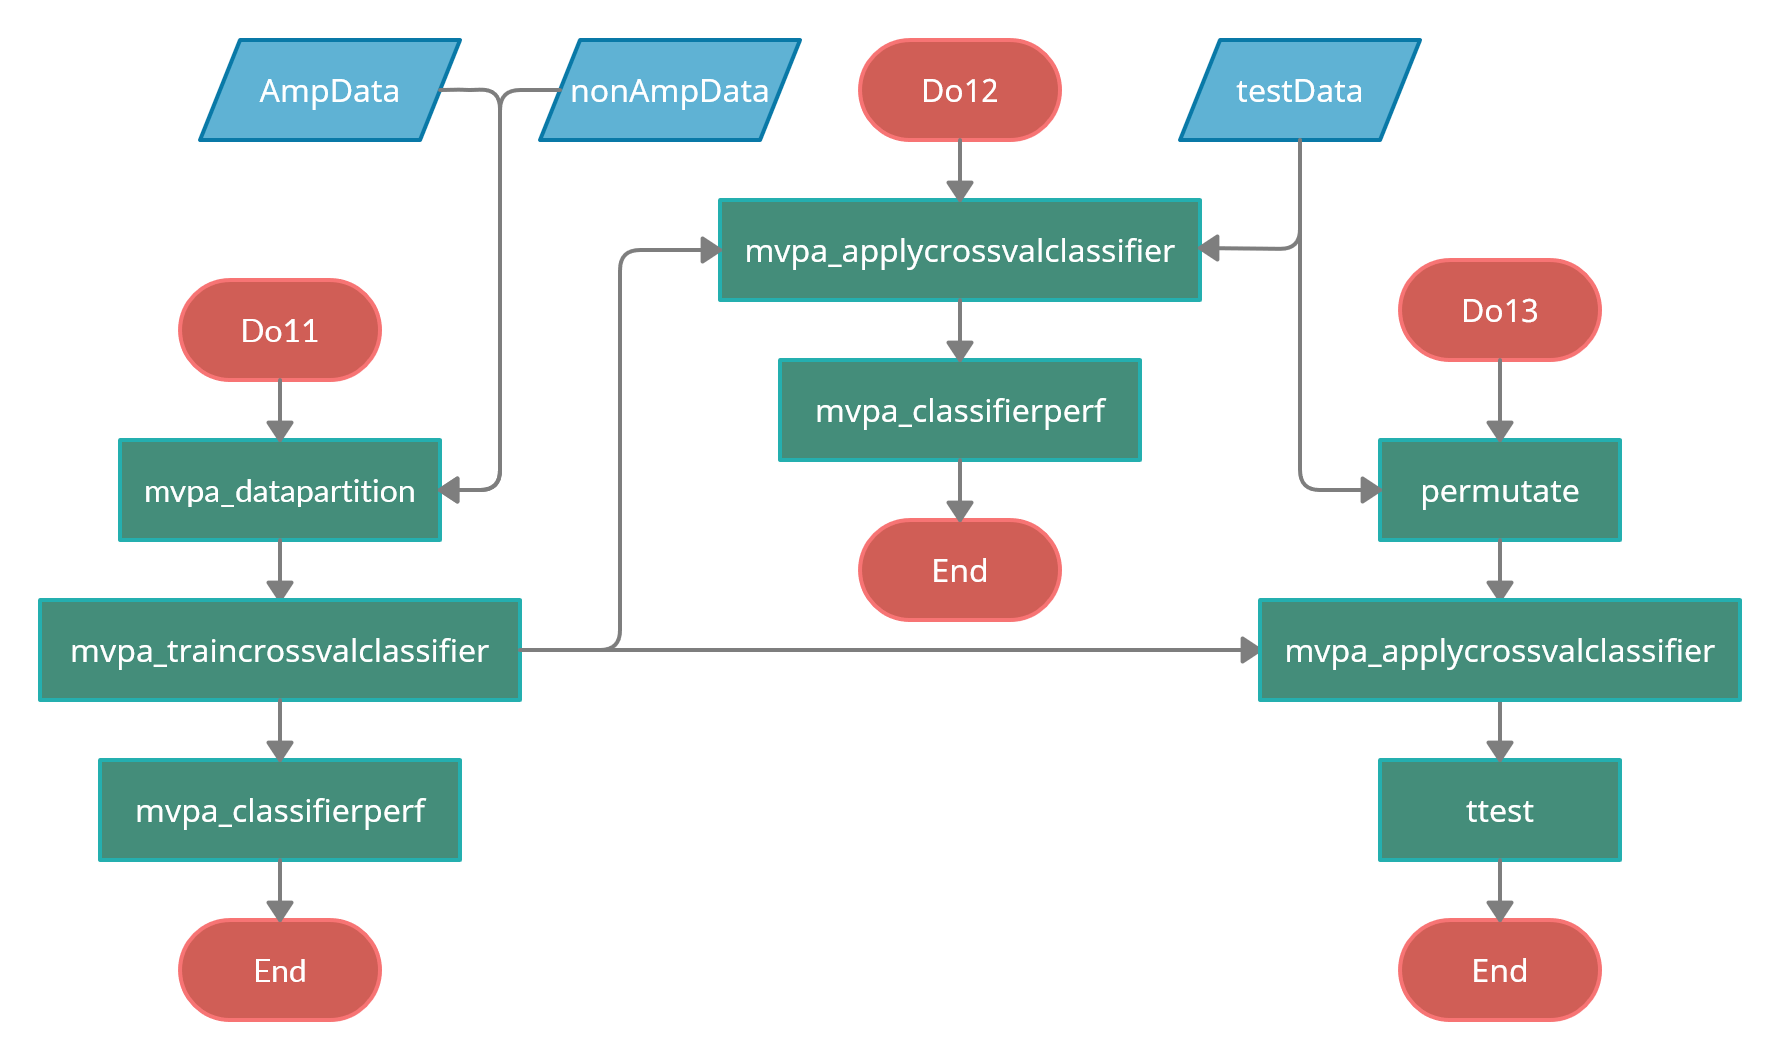
\includegraphics[width=1.0\textwidth, ]{pictures/General structure Master Thesis.png}
    \caption{For simplicity \texttt{Do11TrainClassifier}, \texttt{Do12TestClassifier} and \texttt{Do13TestClassifier\_ShuffledLabels} was shortened to \texttt{Do11}, \texttt{Do12} and \texttt{Do13} in the figure.
    The figure illustrates the execution flow of the program, showing a high level overview with arrows indication input or execution flow.
    Red ellipses mark the beginning or end of a script, a blue diamond marks input data and a green box marks a function.
    Arrows from input data or functions indicate input to another function.}
    \label{fig:GeneralProgramStructure}
\end{figure}

%write an overview of the main scripts maybe

\cref{fig:GeneralProgramStructure} shows \texttt{Do11TrainClassifier} being executed with \texttt{Do12TestClassifier} and \texttt{Do13TestClassifier\_ShuffledLabels} executed in parallel, due to both \texttt{Do12TestClassifier} and \texttt{Do13TestClassifier\_ShuffledLabels} only relying on the results from \texttt{mvpa\_traincrossvalclassifier} in\\
\texttt{Do11TrainClassifier}.
Though the Figure shows \texttt{Do12TestClassifier} and \texttt{Do13TestClassifier\_ShuffledLabels} being executed in parallel they were only executed in parallel in the Ray implementation and Ray does it by default given enough CPUs.
Even if the Ray implementation computes \texttt{Do12TestClassifier} and \texttt{Do13TestClassifier\_ShuffledLabels} in parallel, \texttt{Do13TestClassifier\_ShuffledLabels} needed the results from \texttt{mvpa\_traincrossvalclassifier} for all subjects before continuing.
The reason why \texttt{Do13TestClassifier\_ShuffledLabels} could not process each subject independently was because each t-test was performed over all subjects for each permutation.

\texttt{Do12TestClassifier} could as opposed to \texttt{Do13TestClassifier\_ShuffledLabels} process every subject independently as they finished in \texttt{Do11TrainClassifier}.
Since \texttt{Do12TestClassifier} processes subjects from \texttt{Do11TrainClassifier} individually they help to mitigate the bottleneck of waiting for all subjects to be finished in \texttt{Do11TrainClassifier}.
 

\section{Theory}

\subsection{Cluster Framework}

A cluster computing framework or cluster framework is a framework from which one can set up and schedule computation that are to be distributed and computed over a cloud or cluster of computers.
When refering to a cluster framework henceforth it should not be confused with other frameworks which could be categorized as cluster frameworks.
A cluster framework in other contexts could for example  refer to a framework for virtualizing a cluster of computers to appear as a single machine.
The virtualization of a cluster of computers to appear as a single machine could be used for applications or programs which are written for parallelization on a single machine.
In this project a cluster computing framework does not virtualize a cluster but simply coordinate communication between computers and allow instructions to be executed on those computers.
Distribution of a problem to multiple computers can speed up otherwise slow code if the computations are parallelizable.
The distribution of a problem also has to contend with the communication overhead from sending instructions to other computers in a cluster.
If the communication overhead in a distributed problem is not small compared to the execution time it could be slower to distribute the problem.

In Python there are multiple different libraries which serves as a cluster computing framework~\cite{PythonClusterFrameworks}.
Two of the most popular cluster frameworks are Dask and Ray, both of which are fairly recent projects which are still in active development.
Dask, according to its authors, is a flexible library for parallel computing. 
Dask specialize in processing of large datasets by extending commonly used libraries such as NumPy and pandas, to solve the issue of computing datasets which does not fit in memory for a single node/computer.
Ray is a framework for building parallel and distributed applications with focus on low latency and high throughput scheduling.


\subsection{Ray}

\subsubsection{Ray Overview}

Ray is an open-source project that was developed with primarily machine learning in mind~\cite{nishihara2017realtime, moritz2018ray}. 
Even if Ray was developed primarily for machine learning applications, it is a general purpose framework for distributing computations~\cite{ray:whatIsRay}.
The core functionality of Ray only requires decorating functions with a Python function decorator, meaning it does not require an extensive amount of time to learn.

% write more about dask?
The data processed in this project were all relatively small, thus the main advantages with Dask fell off.

Ray's development team have stated that while they have API (Application Programming Interface) simplicity and reliability as their system design goals, they can give preference to their core system goals, performance and reliability during development~\cite{ray:SystemDesign}.

%Write more in detail about Ray and how it works

%Usage/functionality, finns det någon bättre term?
\subsubsection{Ray Usage}

The main function in Ray enable executing Python functions or classes in parallel with Python function decorators, called remote functions or remote actors~\cite{ray:remoteFunctions, ray:remoteClasses}.
Henceforth remote functions and classes will be collectively referred to as remote functions.
Defining a set of remote functions packages them to be available and executed on a Ray cluster.
A Ray cluster is the background server and services run on a computer cluster by which the computers communicate and send instructions to each other~\cite{ray:rayCluster}.
%Inte bästa citation, se om man kanske kan hitta en bättre source för vad Ray cluster e.
To compute something with a remote function one calls it as a normal function and appends \texttt{.remote} before the arguments. 

Remote functions returns abstract remote objects which represents the results from the remote functions.
By returning abstract remote objects, Ray can schedule and execute other remote functions in parallel with previous and future calls to remote functions.
Execution of a remote function is done in the background asynchronously from the script that called it and other remote function calls, on available hardware resources in the Ray cluster~\cite{ray:remoteFunctions}.
%Kanske ska ha understående mening och byta ut meningen innan förra
%Because execution of remote functions is done in the background and instead returns remote object, a script can call more remote functions to be done in parallel.
Remote objects from remote functions in Ray are mainly used as arguments in other remote functions.
Using abstract remote objects as arguments in other remote functions creates dependencies which Ray takes into account.
Ray schedules and computes dependencies first, executing functions which have dependencies after their dependencies have been computed.
Remote objects used in remote functions act as if they were the results the remote objects represents.
With abstract objects used to represent future results, the intermediate results don't have to be returned to the scheduling node but can instead be either computed on the same node or sent to another available node~\cite{ray:remoteObjects}.

To retrieve a result from a remote object, the method \texttt{.get} is used.
The \texttt{.get} method retrieve and return the result an abstract remote object represents~\cite{ray:FetchingResults}.
When \texttt{.get} is called, the script will block any subsequent function calls and wait until the result is computed.
The Ray developers themselves recommend to delay retrieving results as much as possible because blocking subsequent scheduled remote function calls stops possible parallelism~\cite{ray:delayget}.

Aside from the two main things in Ray, remote functions and \texttt{.get} to retrieve results, there are multiple supported libraries to speed up machine learning or to utilize Dask functionalities for example~\cite{ray:RaySGD, ray:Rayrllib, ray:RayTune, ray:RaySklearn, ray:DaskOnRay}. 
It is possible in Ray to declare resource constraints for each remote function such as memory or CPU, or set up a scheduling strategy to make sure it is properly scheduled~\cite{ray:Resources, ray:PlacementGroup}.
A schedule strategy in Ray could be to schedule things as locally as possible and only use other machines when absolutely necessary, or vice versa.

\subsubsection{Dask versus Ray}

%Lägga till i slutet av Ray/Dask subsection för comparison kanske.
There have been discussions of the differences between Ray and Dask and many have concluded that the scheduling is the main difference between the two.
Dask have a centralized scheduler which maintains and delegates all work, while on the contrary, Ray uses a decentralized scheduler, allowing each node to schedule work on the Ray cluster and within itself.
There are advantages to both Ray and Dask, but Ray should theoretically have a more scalable strategy.


\subsection{The Accelerator}

The Accelerator is a data-processing framework which aims to provide fast data access, parallel execution, reproducibility and transparency~\cite{exax:Accelerator}.
The main advantages with the Accelerator in terms of performance is reproducibility.
Reproducibility means the Accelerator is able to keep track of what source code and dependencies have been used for each execution.
The Accelerator can use old data from already executed code for which new code relies on~\cite{exax:sourceCode}.
Using old data means the Accelerator is skipping code which has already been executed, saving time from unnecessary code execution.
Assuming the execution time is evenly distributed and that the code is evenly changed over time, the Accelerator could on average remove up to 50\% of the execution time from start to finish.
The Accelerator also have parallel execution built in to utilize all of the local CPUs resources~\cite{exax:parallelExecution}.

By letting the Accelerator keep track of what has been executed and when, maintenance of the code becomes automated.
Automating code maintenance speeds up development and eliminates human error which could be critical in a scientific or industrial environment.

%\subsection{Python}
\subsection{General Guidelines for Python Optimization and Speed}

According to Python Scripting for Computational Science by H.P. Langtangen there are a few clear general best-practice rules for optimal run-time performance~\cite{pythonBook}.
%The rules setup by Langtangen are to be viewed as guidelines since they are not universally true and Python as a programming language is due to change further since its publication in 2008.
%Langtangen reccomended to always use if statements but profiling of the Python code showed that an if statement was bottlenecking the code, something which further proves the point that the rules by Langtangen are to be viewed as guidelines.
While the rules setup by Langtangen are great tips, one must remember that optimizing before profiling or when coding is a trap.
Preemptively optimizing before even writing some code could degrade performance or prolong the development time.
It is often better to profile and optimize after writing the first version of the code than to preemptively optimize.

High Performance Python was found in this project to be the better choice compared to Langtangen on how to find slow code and make fast Python code~\cite{oreilly}.
Langtangen and High Performance Python focus on different things however, so it is not a fair comparison.
Langtangen is targeted towards people who when it was published might be considering switching to Python and what they should think about when programming.
High Performance Python is explaining a framework to follow for faster Python code, what parts are most crucial and when to move on with other tools to make Python faster.
It is important to note that while High Performance Python had a greater impact on the speed of the code in this project, Langtangen was also of great importance to the optimizations made.


The useful rules used by Langtangen in this project are listed in the following paragraphs.
Not all the rules from Langtangen have been listed in \cref{guidelines}, the few listed were found to be relevant in optimizations after profiling and made the code remarkably faster.
\begin{itemize}\label{guidelines}
    \item \textbf{Rule 1}: Avoid explicit loops, use vectorized NumPy expressions instead.
    There are several things to the rule, if it is possible and the memory is available a vectorized NumPy operation can see a speedup factor of ten or more as Langtangen describes it~\cite{NumpyArray}.
    Because NumPy will often use more memory than an explicit loop, it could lead to a slowdown rather than a speedup in cases where there isn't enough memory for example~\cite{Numpy:Vectorization}.
    In the end it depends on the circumstances, often the extra memory use in a vectorized solution is negligible compared to alternatives.
    Only profiling can tell if a vectorized solution is faster or not.
    
    The speedup from vectorization in NumPy comes from it using precompiled code in C to do the computations, avoiding the overhead from Python~\cite{Numpy:Fast}.
    The problem of explicit loops being slow in Python stems from the fact that Python is an interpreted language.
    In a compiled language an interpreter does not have to interpret each line of code for every iteration of an explicit loop.
    Just by avoiding interpretation a compiled language has a significant speedup compared to Python because it has to interpret the code.
    A compiler can use other techniques such as loop unrolling to avoid unnecessary instructions or load times~\cite{wiki:LoopUnroll}.
    A compiler is able to notice patterns in loops to better optimize the code structure for the hardware, without changing the final results.

    \item \textbf{Rule 2}: Avoid module prefix in frequently called functions.
    There are two main ways of importing code from other modules/libraries in Python.
    Python can import a whole module with \texttt{import moduleName} or import specific functions from a module with \texttt{from moduleName import functionName}.
    Importing a whole module would require any calls to the functions within the module to be prefixed with its name, also called module prefix.
    For example, if NumPy has been imported with \texttt{import numpy}, constructing an array object in NumPy would be \texttt{numpy.array}.
    Importing specific functions from a module would omit the module name prefix, thus creating a NumPy array would simply be \texttt{array}.
    
    The difference in how imports are made is that there are two different namespaces used depending on how an import is made and this is illustrated in High Performance Python.
    Importing functions using the \texttt{from} keyword sets the function in the global namespace, making accesses relatively fast.
    Importing a whole module in Python with only the \texttt{import} keyword makes any subsequent functions calls do two dictionary lookups, one for the module and one for the function~\cite{oreillyCh4}.
    In theory there shouldn't be a difference between the two methods of importing if only calling a function once.
    
    Even though explicit use of functions are fast, there seems to be a greater overhead for just one function call if a function is imported explicitly compared to importing a whole module.
    %kolla om man ska ha med följande mening, kan vara värt att nämna att det inte var min idé att testa ursprungligen
    %The idea of importing a whole module for functions which are only called once were found in post on \url{https://stackoverflow.com} but couldn't be found for citation.
    The speed difference between explicit imports of functions and a whole module when executing a function once, can easily be made with the timeit module.
    Just to illustrate the speed difference for a single function call, a fast test was done with \texttt{python3 -m timeit -v 'from numpy import array; a = array([0])'} (\SI{1.4}{\micro\second} per loop for 200 000 loops) and \texttt{python3 -m timeit -v 'import numpy; a = numpy.array([0])'} (\SI{986}{\nano\second} per loop for 200 000 loops).

%   \item Rule 3, plain functions are called faster than class methods.
    \item \textbf{Rule 4}: Inlining functions speeds up the code.
    Function calls in general introduce overhead as each time a function is called it has to be looked up in the namespace before executing the code~\cite{oreillyCh4}.
    From a performance point of view it is therefore recommended to just inline small functions, however functions maintain readability and shouldn't be disregarded for small perfomance gains. 

%   \item \textbf{Rule 5}, Avoid using NumPy functions with scalar arguments.

%   \item \textbf{Rule 6}, use xrange instead of range.

    \item \textbf{Rule 7}: \texttt{if-else} is faster than \texttt{try-except}.
    While it is generally always recommended to use \texttt{if-else} over \texttt{try-except} there are exceptions to this rule.
    Profiling of the scripts showed that because of the condition, an \texttt{if-else} statement was taking ten percent of the execution time, see \cref{metodAny}.

%   \item \textbf{Rule 8}, avoid resizing NumPy arrays.
%   \item \textbf{Rule 9}, let \texttt{eval} and exec work on compiled code.
%   \item \textbf{Rule 10}, callbacks to Python from fortran and C/C++ are expensive.
%   \item \textbf{Rule 11}, avoid unecessary allocation of large data structures.
%   \item \textbf{Rule 12}, be careful with type matching in mixed Python-F77 software.
%   \item \textbf{Rule 13}, F2PY may introduce time-consuming copying of arrays.
%   \item \textbf{Rule 14}, Calling C++ classes via SWIG involves proxy classes.
%   \item \textbf{Rule 15}, wrap2callable may be expensive.

\end{itemize}

The list shown in Python Scripting for Computational Science~\cite{pythonBook} are good guidelines, but profiling is to be seen as the first and foremost tool to use and interpret when optimizing Python or any high-level language code for that matter.
The first chapter in High Performance Python go into great detail about profiling and repeat throughout the book that one must continuously profile and interpret the results, both execution and memory usage.
Besides profiling, High Performance Python shows other many different tools such as compiling and clusters to improve performance in Python.
High Performance Python also emphasizes the importance of exhausting previously listed options in itself first, as they are usually what will lead to a higher speedup~\cite{oreillyCh10}.

\subsection{Profiling and Code Optimizations in SW Engineering}

\subsubsection{Profiling}

Profiling in Python was made with the cProfile library.
cProfile is a standard library recommended for most users by Python when profiling code.
cProfile is a library made in C for collecting statistics during runtime with a focus on minimizing the overhead~\cite{Py:cProfile}.
There is another standard Python library for profiling besides cProfile, called profile.
Profile have more features already built in, but is generally less recommended since it runs slower and skews the statistics more when running long programs~\cite{Py:cProfile}.

Profiling in MATLAB was done using the native profiler~\cite{matProfile}.
Both profiling libraries in Python and MATLAB introduces some overhead and certainly to different degrees.
This project however assumed the overhead to be negligible in comparison to execution time and for any comparison between the Python and MATLAB implementation.%Could Expand and discuss the overhead from profiling.

\subsubsection{File Saving}

%add something about different ways of saving due to it being a problem in this project.
Multiple ways of saving Python data was explored during the project due to \texttt{savemat} from the SciPy.IO library bottlenecking the code, which is discussed in \cref{MATPYConv}.


There were multiple ways of saving files, all with different advantages and disadvantages.
One solution that was explored was Apache Arrow, which is a library for storing flat or hierarchical data in a columnar memory format.
Apache Arrow is designed for efficiency on modern hardware like GPUs and CPUs~\cite{AA:apacheArrow}.
According to Apache Arrow, the advantage of a columnar memory format~\cite{enwiki:columnarData} is the use of vectorization operations on data with SIMD (Single Instruction, Multiple Data) instructions included in modern processors.
When data is sorted into columns, multiple entries in a single column could be changed with SIMD instructions~\cite{AA:Overview}.


Because CPUs are much faster than disks~\cite{DiskSlow}, compressing data could be relatively cheap in terms of time in contrast to writing directly to disk~\cite{1607248}.
A smaller file size due to compression decreases the time on the data bus when moving data to disk and the time to write to disk.
Even if smaller amounts of data takes less time on the bus, one must still consider the time it takes to compress the data, the compression ratio and the write speed, most of which depend on the hardware.

Not only CPUs have become increasingly better, a lot of work has been done with storage devices as well.
Modern hardware have tried to move disk closer and closer to the CPU with various means, such as using caches within the disk to be able to read and write data faster to it~\cite{enwiki:1015447262}.
Even if storage devices have improved, it is worth noting that CPUs have improved much faster and will in general always be faster than any other part in a machine.
Most other parts in a machine are slower than the CPU because machines use a memory hierarchy to simulate fast and large storage~\cite{ComputerMemoryHierarchy, enwiki:memoryHierarchy}.
%Ignoring the price of fast storage, there is still a fundamental law of physics which is unavoidable when designing CPUs which is the speed of light.
%The reason the speed of light is important is because electricity moves at the speed of light and CPU clock frequencies today can be up to \SI{8}{\giga\hertz}.
%The length speed of light moves between one clock cycle at \SI{8}{GHz} is about \SI{4}{\centi\meter} ($c/3GHz$) which is the theoretical maximum, not accounting for other factors which decreases the length traveled in a CPU.
With the CPU being much faster than disk, it is sometimes worth investigating things such as data compression for a better runtime performance.

The implementation of Apache Arrow's save format was however left as an in depth problem due to the time saving files becoming negligible after using pickle.
pickle is a standard library in Python for serializing and saving files in Python~\cite{Py:pickle}.

\subsubsection{Extension Modules}
%After removing the problematic \texttt{savemat} new profiling was made, identifying unnecessary code, parts which could be replaced with a faster extension module or more optimized Python code.
For a high level scripting language such as Python, anything done in an extension module is almost always faster.
Extension modules in Python are usually faster because they are usually written in a faster language such as C~\cite{cFaster}.
Modules written in Python are usually also faster as they are developed over time by a larger team with a userbase who have interests in using fast and optimized modules.

\subsubsection{Writing Functions}

Even with the extensive community behind Python there will still be things that cannot be exchanged with an extension module.
One such problem was reorganizing two lists of which one mapped a class to the other's data.
A problem with potential solutions to reorganizing two lists was doing a good complexity analysis.
Growth complexity in high level languages such as Python become intricate as a function which might have a faster growth theoretically is often still faster if it is computed at a lower level, compared to a function computed at a higher level with a slower growth.
The final solution to mapping classes to data had a growth of $\mathcal{O}(n\log n + k)$, see \cref{stackSolution}.
A linear solution written in pure Python was possible but the advantage with the final solution was that both terms were fast due to using NumPy.
NumPy is written in C~\cite{Numpy:Fast}, bringing down the computations to a lower level and making things which at the surface seems slower much faster.
%%Write more here.
\newpage
\lstinputlisting[language=Python]{Scripts/mvpa/ArrGroupLabel.py}\label{stackSolution}
%Write muchos more about it 

\subsubsection{\texttt{if-else} versus \texttt{try-except}}

A function which was found to be unnecessary was an \texttt{if} condition checking that all elements in an array were not empty, see \cref{metodAny}.
Checking if an array is empty is slow both in Python and MATLAB as it has to iterate through every index or check if it exists.
Even if an \texttt{if} statement was shown to be at fault here, it is exceedingly rare and should be viewed as the exception.
\texttt{try-except} is slower than \texttt{if} statements~\cite{pythonBook} and raises the problem of having to deal with exceptions which are expected but might be raised where they are unexpected.
Exceptions are slow and expensive therefore it is imperative to be careful if one uses \texttt{try-except} instead of an \texttt{if} statement.
The extra overhead from exceptions can degrade performance more than just using an \texttt{if} statement it is therefore important that the majority of the time there aren't any exceptions or that the alternative is exceedingly slow.
It is in general advised to use \texttt{if} statements since Boolean expressions are usually fast operations.

\subsubsection{Looping}

\texttt{for} loops in Python are usually very slow because each iteration is reinterpreted since Python does not compile the code.
Something which could speed up loops in Python are for example \texttt{map}, \texttt{filter} or list comprehensions~\cite{Py:map, Py:filter, Py:listComprehension}. 
For \texttt{map}, \texttt{filter} and list comprehensions the expressions are interpreted once and then computed for the whole loop, theoretically saving several iterations of interpretations for the same code.
There does not seem to be a definitive answer to what is faster between ordinary loops, map, filter or list comprehensions though.
In the end when it comes to Python one must follow profiling for everything to see what is fastest.

%Should I have code here with the critical part of the code?
\subsubsection{Lookups}

Python lookups are a small set of optimizations but exists everywhere in Pythono.
Just a simple function call is a lookup to where the function is located.
It is debated if people should even think about lookups since there are usually much larger speedups in either using another lower level language or in compiling the code.
Just as there are a different number of lookups depending on how the import of a module is done, there is a lookup for each layer of a nested Python object.
A way to avoid multiple unnecessary lookups for nested objects in loops is to save each layer as a temporary variable to reference.
While most of the things mentioned might be micro-optimizations and often not meaningful by themselves, they add up.
However the most critical optimization in the project was due to lookups.
%Need to extend these two sentences, feels a bit weak.
%Expand on how the feature reduction might be unnecessary. Could be interesting to compare.

%APPEND THIS SOMEWHERE%%%%%%%%%%%%%%%%%%%%%%%%%%%%%%%%%%%%%%%%%%%%%%%%%%%%%%%%%%%%%%%%%%%%%%%%%%%%%%%%%%%%%%%%%%%%%%%%
Without resorting to clusters the final solution for making any Python code faster would be to compile the code using a third party compiler such as Numba or Cython~\cite{matEval}.
Compiling was not implemented in the project as it was concluded that it might just add another layer of complexity which the researchers will have to learn.
Ray does support Cython code to speed up computation so it would have been possible to see an even greater speedup than the results of this project.


%Not sure if I wanna keep this or not->
%Even with all the mentioned changes it must be noted that the incessant loading and saving of files between scripts was creating excessive overhead, a small optimization step was to skip all intermediate loading of files.



%\subsection{Algorithm, memory approaches}
%Wasnt really a question of optimizing any algorithm
\subsection{Conversion Between Languages}

Conversion from MATLAB to Python have shown to be almost entirely supported by the immense amount of modules for Python.
Many of the solutions used in science which are available in MATLAB are already supported by the module NumPy and most machine learning is supported with \textsl{scikit-learn} in some form.
With a vast array of machine learning models supported in Python it is not weird that almost all cutting edge machine learning research publish their models in a Python module in some form.
Since all new machine learning models are usually available in Python, it is the preferred language for implementing research using machine learning~\cite{Silaparasetty2020}.

This project found the limiting factor for conversion from MATLAB to Python to be a lack of documentation or insufficient details in documentation to be able to reproduce identical results.
Different languages can implement identical functions differently creating small differences in the results citation.
Due to differences in implementation for near identical functions, a cascade of larger differences could be created at the end of a program.
%Ska jag lägga till några exempel om vad som va annorlunda, kanske citera nånting och visa att de e implementerade annorlunda.
Because of the small differences in implementation, documentation becomes vital when trying to convert programs.
For example the Python and MATLAB libraries for EEG processing, FieldTrip and MNE, have different approaches in processing~\cite{MNEVersusFielder}.
A large part of why the preprocessing scripts were not translated were because of the differences between FieldTrip and MNE. 
A reason why one do not usually translate code and instead redo the whole program from scratch, is that even seemingly identical and standarized models such as SVMs can be implemented differently.
Seemingly identical libraries are implemented differently, in different languages for a vast array of reasons, from different developer teams to how the languages themselves work.


\subsection{Code Parallelization}

Parallelization refers to the conversion of sequential code to utilize multiple processors or vector instructions to execute multiple instructions in parallel.
Classically, CPUs execute instructions in order one after the other, however with the introduction of multiple cores in computers, instructions which are independent could be executed in parallel.
Parallelization does not always have a straight forward solution and code often has to be manually parallelized.
Parallel code is often implemented sequentially first and then converted to be parallel, in other words parallelized.
%With code often being implemented sequentially first, parallel code have often been converted and thus parallelized.

Even if a problem is parallelizable it is not always the best course of action to use a cluster if there are no reasons to do so.
The execution time of having to distribute a problem to an entire cluster has to outweigh the original execution time.
Because CPUs are extremely fast the communication overhead from distributing work to other CPUs often makes a program slower than running everything on the same CPU.
There's even a small communication overhead in parallelizing problems on the same CPU, it is however not usually something one has to consider.
%Because of the communication overhead, not all independent layers of the code were parallelized.
%Another reason was to avoid unnecessary complexity since the potential performance gains were deemed negligible compared to the readability.

%Detta skall nog vara i metoden
%The strategy used to parallelize was quite straightforward. 
%The code processed 18 independent subjects, the data from each subject was then partitioned into several independent %datasets with for-loops and trained models on each of the independent partitioned datasets. 
%Because the subjects and the partitioned datasets were independent they could be processed in parallel instead of sequentially, making it the obvious part of the code to parallelize.
%The framework called Ray was used to parallize the code. 

%With Ray's abstraction of objects and no real dependency between large blocks in the code, a large advantage with Ray emerged as \texttt{.get} could in practice be delayed until the end.
%With no need to retrieve intermediate results the full potential of Ray emerged, filling all cores in the cluster with work for the duration of the scripts.
%When delaying the get function, the Ray scheduler can schedule things as computer resources are freed up and required data is available.
%Ray does not need to return unnecessary intermediate data, instead it returns a remote object, a promise of a future which Ray can use as if it was the object itself when sending to another remote function.
%Ray's abstraction of objects creates a more distributed execution of the code and utilizes all of the available hardware.

\subsubsection{Ray}\label{RayNesting}

After the first layer of parallelization was implemented, further work on multiple layers of parallelization proved more problematic.
While Ray excels at large parallelization there still exists problems with nesting remote functions. As such, workarounds had to be made to solve the problems.
The biggest with nesting remote functions in Ray is when the \texttt{.get} method is called it signals to the Ray scheduler that it is no longer using hardware resources.
If \texttt{.get} is used within a remote function Ray will see it is no longer using resources and execute the next scheduled function, thus potentially executing more functions than there is CPU cores or memory.
Even if there are ways of avoiding nesting remote calls, the unnecessary workarounds could lead to degradation and hopefully the Ray developer team fixes this feature. 

\subsubsection{Amdahl's Law}

Amdahl's law states that the bottleneck of parallelizing a program will always be the serial part of the code, in \cref{Amdahl} $S_{latency}(s)$ is the total speedup of a program after parallelizing, $p$ is the fraction of the whole program which is parallelizable and $s$ is the speedup of the parallelizable part of the program.
The implication of Amdahl's law is that if eighty percent of a program is parallelizable, the program can at most be cut down to twenty percent of the original execution time given an infinite amount of cores due to the twenty percent which must be done serially.

\begin{equation}\label{Amdahl}
    S_{latency}(s) = \frac{1}{(1-p) + \frac{p}{s}}
\end{equation}

\subsection{BLAS}

BLAS (Basic Linear Algebra Subprograms) are libraries for accelerating linear algebra operations.
This project found that the precompiled BLAS libraries from NumPy was slowing down the code, see \cref{inPara,AppendixSeperateTimes}.
BLAS libraries are usually compiled to use the available cores on a computer to speed up computations, since linear algebra operations are often parallel by nature.
Having BLAS utilize all of the hardware should theoretically decrease the computational time enormously.
However the project found that the code used in the project slowed down both in a sequential and parallel environment when BLAS was using all cores, see \cref{Acc:NumPy1Thread,AppendixSeperateTimes}.
%While in day to day programming having BLAS utilize all of the hardware is usually an extreme boost in decreasing execution time, it can bottleneck a problem which is otherwise trying to occupy all the threads.

There could potentially be many problems in fighting over hardware resources, for example hardware predictions could be harder as the CPU has to switch between the different instructions.
Conflicting instructions from different threads could cause a higher demand in memory.
A higher demand in memory could lead to the CPU having to resort to a lower level in the memory hierarchy to fetch the data for computations etc. 
There are an array of troubles which could decrease performance when fighting over hardware resources.
These are all speculations however and no deeper analysis as to why BLAS was slowing down the code was made.
%The test results from testing if BLAS was slowing down the code are presented in \cref{AppendixSeperateTimes}.
While there is an enormous boost to do simple vector operations in parallel, all modern CPUs have solved the main issues with vectorization operations by implementing fundamental vectorization instructions in the CPU which optimizes these operations for a single core~\cite{enwiki:avx}.

\subsection{Error Estimation and Computations}

The speedup factor when scaling up from one machine in Ray was calculated by dividing the execution time of using one machine in Ray with the execution time of using $n$ number of machines, where $n$ is between one and twenty five machines.
The speedup equation can be seen in \cref{speedupFac}, $f_{speedup}$ is the relative speedup compared to using one machine, $t_1$ is the mean execution time of using one machine in Ray and $t_n$ is the mean execution time of using $n$ machines.

\begin{equation}\label{speedupFac}
    f_{speedup} = \frac{t_1}{t_n}
\end{equation}

Standard deviation and mean of the time measurements were calculated using NumPy's std and mean functions.
All measurements were assumed to be independent.
Because cProfile does not specify the time resolution, no time resolution for the time measurements were included in the calculations.

Since the measurements were assumed to be independent, the speedup factor of Ray compared to one machine used propagation of uncertainty seen in \cref{stdProp,ErrorProp} to compute the relative error.

\begin{equation}\label{stdProp}
    s_f = \sqrt{\left(\frac{\partial f}{\partial x}\right)^2s_x^2 + \left(\frac{\partial f}{\partial y}\right)^2s_y^2 + \cdots}
\end{equation}

\begin{equation}\label{ErrorProp}
    \begin{aligned}
        s_{speedup} &=  \sqrt{\left(\frac{\partial f_{speedup}}{\partial t_1}\right)s_1^2 + \left(\frac{\partial f_{speedup}}{\partial t_n}\right)s_n^2} \\
        s_{speedup} &= \sqrt{\left(\frac{1}{t_n}\right)^2s_1^2 + \left(\frac{-t_1}{t_n^2}\right)^2s_n^2}\\
        s_{speedup} &= \sqrt{\frac{s_{1}^2t_n^2 + s_{n}^2t_1^2}{t_n^4}}
    \end{aligned}
\end{equation}

Assuming variables are independent, the equation for propagation of uncertainty is as seen in \cref{stdProp}.
Using \cref{stdProp} the propagation of uncertainty for \cref{speedupFac} is as shown in \cref{ErrorProp}.
$s_{speedup}$ in \cref{ErrorProp} is the standard deviation of the speedup factor, $s_1$ and $s_n$ are the standard deviations of the execution times for using one machine and n machines respectively.

The total execution time of non Ray implementations were calculated by adding each individual script's mean execution time.
The standard deviation of the total execution time was calculated by adding each individual scripts standard deviation, following the standard way of calculating propagation of uncertainty.

\section{Methodology}

\subsection{Rewriting MATLAB}

Upon retrieval of the MATLAB code it was executed to ensure it was working as intended.
The number of iterations in \texttt{Do13} was decreased from five hundred to a hundred to decrease the execution time in testing and during development of the Python code.
After execution, the code was read thoroughly to understand how it was constructed and what was happening.
The MATLAB code was profiled to have an overview of performance and potential bottlenecks.
The first profile would serve as a baseline for the project.

Since all of the main scripts were mostly written using the native \texttt{eval} function from MATLAB, they were first translated to basic code.
\texttt{eval} is a built in function in MATLAB which evaluate string values as MATLAB expressions~\cite{mat:eval}.
There are many reasons to avoid \texttt{eval} and while it allows for some interesting interactions it is safer, faster and easier to read code which do not use eval.
MATLAB usually compiles code the first time it is run but it is not possible with \texttt{eval}.
\texttt{eval} is not safe, it could for example unexpectedly overwrite variables with new values~\cite{matEval}.
Since \texttt{eval} evaluates string values, the arguments will be monochromatic because they are string values.
Reading code which is not properly color coded and instead monochromatic, decreases the readability significantly.

The removal of the \texttt{eval} functions increased readability, and made later translation to Python easier. With no \texttt{eval} operations the syntax was color coded and much more distinguishable when jumping between MATLAB and Python code.
Removing \texttt{eval} also allowed for basic parallelization in MATLAB, using the \texttt{parfor} function from the Parallel Computing Toolbox in MATLAB.
The parallelization of the preprocessing code of MATLAB was very briefly explored and quickly left as an in-depth problem for future work.
Removing \texttt{eval} and parallelizing the preprocessing scripts with \texttt{parfor} in MATLAB seemed to show a significant speed up.
The parallelized preprocessing scripts were unfortunately never confirmed to work as intended before leaving it for future work.
%Apart from assuring the parallelized preprocessing scripts were working as intended, the parallelization of the preprocessing scripts were outside the scope and focus of the project so the results were left out.
%Unecessary sentence no?down below
%\texttt{eval} makes any potential compilation impossible since it is not explicit, it can utilize dynamic variables for example.

The largest overhead after implementing \texttt{parfor} was the loading of large data. 
MATLAB was able to avoid the large time penalty of loading from disk for most of the preprocessing scripts.
Despite a significant improvement in performance when using \texttt{parfor}, it did not scale well with the number of threads used.
In the end however the focus of the project was not to optimize the MATLAB code but rather the Python implementation.


\subsection{MATLAB to Python Translation}\label{MATPYConv}

The execution time of the preprocessing scripts were significantly less than the training of the classifiers and permutation of data. 
The necessary literature and theory behind understanding the preprocessing scripts in order to fully translate them was deemed not to be of focus for this project.
FieldTrip, the EEG processing library used in the MATLAB preprocessing scripts and its counterpart in Python, MNE, are not implemented nor process data the same way.
To translate the preprocessing scripts would have required an in-depth knowledge of both EEG processing libraries and a considerate amount of development time.
Because of the low execution time and lack of knowledge it was decided the preprocessing scripts were not to be translated to Python.

Apart from the preprocessing scripts, the MATLAB code was first translated line by line to Python, as close to the original code in MATLAB as possible.
The data from the MATLAB preprocessing scripts were loaded using the SciPy.IO module, which supports loading .mat files.
For the majority, the translation was a matter of reading documentation between the equivalent functions in Python and MATLAB.

Implementing an identical training for Python's SVM proved difficult.
Because MATLAB does not explicitly show how they implement SVM, it is hard to tell what the differences were between MATLAB's implementation of SVM and Python's.
While some of the settings were the same for MATLAB and Python's implementation of SVM, it seems that the difference lies with how the respective error functions are written.
Python's scikit-learn package does allow someone to write their own error function, however it is no clear from MATLAB's documentation how the default error is calculated. %This might be more of constraints issue, from BoxConstraint Try and elaborate on the ERROR, find sources

\subsubsection{Python Slower Than MATLAB}

After implementing a working SVM in the Python code a profile was made of the code using the cProfile module.
After profiling the Python code with the cProfile module, it was found to be three times slower than the MATLAB counterpart.
The reason why the Python code was three times slower was found to be SciPy.IO's built-in \texttt{savemat} function, which took more than sixty nine percent of the computational time.
The large overhead from savemat could be because it did not save as version 7.3 and above, which compresses the data first.
The compression was however quickly disregarded as the original MATLAB code did not use 7.3 and above either.
Since the issue of saving in .mat format did not exist in the MATLAB scripts the problem in Python could have been a multitude of potential causes.
One potential cause could have been because MATLAB already stores the data in .mat format in memory, it was the conversion of the datastructures from Python to .mat format which caused the overhead.
Because the total amount of data saved was somewhat large (>50 GB), it could be SciPy.IO's \texttt{savemat} is slower than MATLAB's native saving which was exacerbated by the large data. 
As the overhead was quite massive it was probably due to a mix of things, which made \texttt{savemat} inefficient in this project.

There were however a few ways to improve the execution time if theoretically keeping the .mat format was important.
An example of improving \texttt{savemat} in Python could be to use the compression option.
A thing which could improve \texttt{savemat} could be to use HDF5 format option, which MATLAB versions above 7.3 uses~\cite{Mat73HDF5}.
HDF5 is built to be a fast way of storing large amounts of data~\cite{WhatIsHDF5}.
HDF5 was never implemented though since it was not necessary to save in .mat format.
Instead of using \texttt{savemat}, files were saved using the Python module pickle.
After switching to pickle to save the files, the time consumed saving files dropped to a fraction of the execution time for the Python scripts.
Switching to pickle decreased the computational time for the \texttt{Do11TrainClassifier} script to half of the MATLAB counterpart. %%Shuffle away this to Python side

Of course the problem of saving in .mat format was not a problem in the MATLAB scripts, but rather something introduced in the conversion to Python and thus something which should not have been there in the first place.

\subsection{Optimization of Python}
The first steps in optimizing after removing \texttt{savemat} was profiling the code again using cProfile.

After profiling the Python code the main issues were identified to be NumPy's \texttt{any} and \texttt{in1d} functions.
NumPy's \texttt{any} function was able to be cut out using \texttt{try} and \texttt{except} statements, skipping the \texttt{if} statements all together.%%Good thing to have in theory.

Due to the highly nested and long \texttt{for} loops in the original code, small performance gains were found in using the built in \texttt{map} function in Python.

\subsubsection{The \texttt{any} Function}\label{metodAny}

Profiling of the scripts showed that a specific \texttt{if-else} was taking ten percent of the execution time.
It was revealed that the reason behind the ten percent overhead from the \texttt{if} statement was due to its condition, using the \texttt{.any} function in NumPy for a NumPy array.
So it was not the \texttt{if-else} statement itself but rather the \texttt{.any} function determining if the condition was true or false.
The \texttt{.any} function can be extremely slow because it has to look through an entire list or determine if the list exists before determining the result.

The \texttt{if-else} were replaced with \texttt{try-except} and after profiling the code again the ten percent overhead was gone.
This was a rare occurrence where profiling revealed that \texttt{if-else} was slowing down the code.

\subsubsection{The \texttt{in1d} Function}

Profiling revealed that \texttt{mvpa\_applycrossvalclassifier} in \texttt{Do13} was using eighty one percent of the time in \texttt{in1d}.
The script \\\texttt{mvpa\_applycrossvalclassifier} used \texttt{in1d} to find the index of multiple elements in a list which mapped sensor names to its index, over two hundred times.
Linear searches like \texttt{in1d} are generally avoided because of the linear growth and it is advisable to find faster solutions if possible.
\texttt{in1d} was removed and replaced with a hashmap which used each sensor name as the key and each index corresponding to the sensor name as the value.
With each index mapped to its element as the key, each lookup became fast and constant.
The execution time previously dominated by \texttt{in1d} in \texttt{Do13} with eighty one percent, dropped to less than a percent when using a hashmap.

\subsubsection{Other Optimizations}

Most other significant improvements were made by finding NumPy functions which replaced parts of the code, to bring down the level where it was computed.
Switching the implementation used to train the SVMs from sklearn.SVC to sklearn.LinearSVC saw a large performance improvement.
libSVM uses another lower level library compared to SVC and is potentially faster for problems with a larger set of features~\cite{LinearSVC,SVMSVC}.

\subsection{Why Ray}

%Ska jag ha understående stycke, kanske inte hör hemma med teorin.
Ray was robust, easy to learn and the fact that Ray had a focus on machine learning made it seem a good choice for the project.
The scientists at Lund University could potentially learn Ray with relative ease and because it is robust, experiment with the framework for future projects.

With Ray being relatively new and having high support for different machine learning libraries to distribute the workload, it seemed both an exciting and good choice in the beginning of the project~\cite{ray:RaySGD, ray:Rayrllib, ray:RayTune, ray:RaySklearn}. 

\subsection{Transition to Parallel Code}
After translation of the original MATLAB code the Python code was
rewritten into a single script.
With the transition into a single script, intermediate loading of files saved from previous scripts could be removed which in turn decreased the execution time a small bit.

To create a more persistent storage of data between creation and deletion of clusters the OpenStack object storage on Ericsson's cloud was used.
Both preprocessed and intermediate data was saved in the OpenStack object storage, to collect all data in a central and easily accessed location.
With OpenStack's object storage Ray could save data remotely without knowing where the master node was.

\subsubsection{Ray}

With Ray the process to transition the code to use the cluster resources over a local network was fast, and done by adding a \texttt{@ray.remote} decorator for the function which was to be computed in the cluster.
A first layer of parallelization over the independent subjects were created using Ray's remote function.
Since there is no dependency in processing the subjects this was a perfect first place to start parallelizing, assuming the computational time for each subject was about the same so that it would not create a bottleneck.
The problem with only parallelizing over the number of subjects was that there were only eighteen subjects and the number of available cores within the cluster was twenty, thus new implementations needed to be more scalable.
%Because there were only eighteen subjects and at the time there were twenty cores available, further work for a more scalable implementation had to be done.
Because the first layer of parallelization saw a dramatic decrease in execution time, the original execution time of a few days compared to the new execution time under an hour led to questioning the communication overhead.

First a more scalable solution with nested functions was created, it was quickly discovered to be problems with nesting remote functions, see \cref{RayNesting}.
The known problem with nested functions led to a small redesign from the original code after a long time of experimental implementations. 
Ultimately, it was possible to avoid the larger issues with multiple layers of parallelization, instead of nesting the remote calls they were made shallow so only a single layer of remote calls were made.
By having a single layer of remote calls the nesting problem was removed and flipped on its head, instead scheduling the smallest part of parallelization without doing any slow work on the main thread.
In the end a fast and working solution was implemented without any noticeable difference in the end results.

\subsubsection{Communication Overhead}

The purely serial parts of the program were well below a few minutes and the time limit of the Ray implementation seems to be around fifteen minutes, see \cref{TotTime}.
The hard fifteen minute limit is probably due to multiple reasons.
The excessive saving of intermediate files in the Ray implementation makes one question the data rate of the OpenStack object store, as each extra core added another connection which wanted to upload data. 
The communication overhead of having to scale the work for more cores and the data rate of sending data between nodes could have been potential bottlenecks.
Finally Amdahl's law assumes a parallelizable part of a program always benefits from more cores, which is not true for most programs.
Parallel programs are usually only parallelizable to the extent in which there is a smallest part of a program which must be done serially.
With other words a program cannot be chopped up into infinite many parts, there will parts which need to be done one after the other.
It could have been the smallest part of the code in the Ray implementation was a factor to the fifteen minute limit.

\subsection{Inherent Parallelization}\label{inPara}

After implementing the Accelerator distributing the problem locally on one machine using all its threads, it was found using Linux's top command that the seperate threads were trying to use more than the assigned thread.
After researching the problem it was found that NumPy was the culprit.
Even though Numpy itself is not multithreaded, it is built on top of precompiled BLAS (Basic Linear Algebra Subprograms) libraries and do not control how the BLAS libraries use the hardware available~\cite{Numpy:OpenBLAS}.
Most BLAS libraries are compiled to utilize as many cores as possible as most operations are extremely parallelizable, NumPy itself come with a precompiled library which uses available cores.
Because NumPy uses multiple threads by default it does not take into account the rare case when someone actually wants to manually parallelize a problem. 
BLAS libraries and NumPy are not aware if they are in a multi-threaded environment or not and has to be manually set to use only one thread~\cite{OpenBLAS:threadSafe}.

This was not a problem in Ray because the Ray development team has noted this problem and solved it temporarily until NumPy's development team fixes it.
Ray's development solved the problem with BLAS during runtime, by changing the environment variable for the most common BLAS libraries to specifically use one thread~\cite{ray:OMPNUMTHREAD}. 
The same fix used in Ray to instruct the BLAS libraries to use one thread was applied to the Accelerator.
The Ray fix was not implemented for the single thread implementations as MATLAB also utilized multithreading for some linear algebra operations.
The Single thread implementations were however tested with BLAS only using one thread and the results shown in \cref{AppendixSeperateTimes} are clear, the native BLAS libraries in NumPy are bottlenecking the code.

Two runs on two different machines were done with the Accelerator implementation, one with NumPy using all threads and one with NumPy only using one thread for a total of four runs.
The results from the four runs are shown in \cref{Acc:NumPy1Thread}.
The runs were done to find out if NumPy might be bottlenecking the code, after it was found out NumPy was trying to use more threads than were available in a multi-threaded environment.

\subsection{Profiling and Measuring}

The final results were generated on 4 VCPUs @ \SI{2.6}{\giga\hertz} and \SI{8}{\giga\byte} memory computing nodes in Ericsson's cloud, with the exceptions of two of the single thread tests.
A comparative single thread test between MATLAB and Python was executed on my personal PC with 8 logical cores @ \SI{3.40}{\giga\hertz} and \SI{36}{\giga\byte} memory, due to memory and license limitations. 
A single thread test for Python was executed on one of the computing nodes to show they were in the same order of magnitude as the test on my personal PC.
The single thread Python test on the computing node was also done for a fair comparison between MATLAB and Python.

All execution times for Python were extracted using cProfile, the execution times for MATLAB were extracted using the built in Profiler.
An exact timing and profiling for each script in Ray was not possible to achieve as the Ray implementation integrated the scripts.
The integration of the scripts in Ray made it possible to compute parts of later scripts as soon as parts of the previous scripts finished.
Because the scripts were integrated and due to how Ray handles scheduling there is no definitive boundary between the scripts and therefore it is only possible to specify the total execution time.

After realizing that the first twenty VCPUs originally assigned and used in this project still scaled well, another eighty VCPUs for a total of a hundred VCPUs were used. With the hundred VCPUs the scalability of the current Ray implementation could be cemented as the time converged to around fifteen minutes, see \cref{TotTime,fig:MachineXSpeedup}.

\section{Results}

The final results are presented in \cref{TotTime,AppendixSeperateTimes} for comparison.
The execution times for Ray do not include the time it takes to set up the cluster nodes or start the Ray cluster.
The results only present the execution times of the Python and MATLAB scripts.
There are multiple ways of managing and setting up a Ray cluster some of which are almost instantaneous, and others which are slower. 
%\texttt{Do11TrainClassifier}, \texttt{Do12TestClassifier} and \texttt{Do13TestClassifier\_ShuffledLabels} in \cref{TotTime} are N/A for the Ray implementation as they are integrated without being able to specify an exact boundary between the scripts.

%Table over execution times for single, thread, accelerator, and Ray implementation
\begin{table}[H]
    \centering
    \caption{Table of the total execution times for the translated and converted scripts as well as the total comparative speedup factor between the implementations, with 1 Thread (MATLAB) as the default speed.}
    \begin{tabular}{|l|l|l|}
    \hline
    \#                 & \SI[parse-numbers=false]{Total}{(\minute)}        & \SI[parse-numbers=false]{Speedup}{(AU)}       \\ \hline
    1 Thread (MAT, PC) & 3426.85$\pm$550.14 & 1.0$\pm$0.23     \\ \hline
    1 Thread (Py, PC)  & 283.63$\pm$1.51    & 12.08$\pm$1.94   \\ \hline
    1 Thread (Py)      & 809.62$\pm$188.22  & 4.23$\pm$1.20    \\ \hline
    True 1 Thread (Py) & 608.48$\pm$42.95   & 5.63$\pm$0.99    \\ \hline
    Ax 4 slices        & 121.77$\pm$13.25   & 28.14$\pm$5.46   \\ \hline
    Ray 1 Nodes        & 174.33$\pm$34.50   & 19.66$\pm$5.01   \\ \hline
    Ray 2 Nodes        & 68.06$\pm$6.55     & 50.35$\pm$9.42   \\ \hline
    Ray 3 Nodes        & 46.29$\pm$5.13     & 74.02$\pm$14.44  \\ \hline
    Ray 4 Nodes        & 35.15$\pm$3.13     & 97.48$\pm$17.89  \\ \hline
    Ray 5 Nodes        & 28.78$\pm$2.46     & 119.09$\pm$21.65 \\ \hline
    Ray 10 Nodes       & 17.58$\pm$0.49     & 194.94$\pm$31.76 \\ \hline
    Ray 15 Nodes       & 16.05$\pm$0.82     & 213.55$\pm$35.97 \\ \hline
    Ray 20 Nodes       & 15.70$\pm$0.61     & 218.29$\pm$36.06 \\ \hline
    Ray 25 Nodes       & 15.83$\pm$0.79     & 216.47$\pm$35.84 \\ \hline
    \end{tabular}
    \label{TotTime}
\end{table}


\begin{table}[H]
\centering
    \caption{Table of the separate execution times for the MATLAB, Python and Accelerator scripts.}
    \begin{tabular}{|l|l|l|l|}
    \hline
    \SI[parse-numbers=false]{\#}{(\minute)}    & Do11             & Do12           & Do13               \\ \hline
    1 Thread (MAT, PC) & 410.56$\pm$12.24 & 29.51$\pm$3.39 & 2986.77$\pm$549.99 \\ \hline
    1 Thread (Py, PC)  & 172.29$\pm$1.24  & 1.35$\pm$0.33  & 109.98$\pm$0.80    \\ \hline
    1 Thread (Py)      & 302.17$\pm$45.64 & 4.53$\pm$0.78  & 502.92$\pm$182.60  \\ \hline
    True 1 Thread (Py) & 313.55$\pm$35.05 & 3.49$\pm$0.39  & 291.44$\pm$24.82   \\ \hline
    Ax 4 slices        & 60.99$\pm$9.10   & 0.81$\pm$0.15  & 59.96$\pm$9.62     \\ \hline
    \end{tabular}
    \label{AppendixSeperateTimes}
\end{table}


Since the MATLAB scripts were run on a different machine than the Python implementations, the single thread Python implementation was run on both the machine everything else was run on and the same machine as the MATLAB script, for comparison.
The tests were performed with a hundred permutations in \texttt{Do13TestClassifier\_ShuffledLabels} although the researchers at Lund University used five hundred permutations in their research.
With five hundred permutations the execution time will converge more towards the comparative speedup of \texttt{Do13}.
To put the comparative speedup factor of \texttt{Do13} into context, it is around twenty seven times faster and \texttt{Do11} is around three times faster in the single thread Python implementation, see \cref{AppendixSeperateTimes}.


%Seperate Table over speedup compared to original MATLAB script?
\begin{table}[H]
\centering
    \begin{tabular}{|l|l|l|l|l|}
    \hline
    \SI[parse-numbers=false]{\#}{(\minute)} & Total & Do11  & Do12  & Do13  \\ \hline
    Xeon all Threads                        & 98.2  & 16.2  & 0.85  & 81.1  \\ \hline
    Xeon 1 Thread                           & 34.7  & 16.3  & 0.21  & 18.2  \\ \hline
    EPYC all Threads                        & 64.9  & 5.6   & 0.6   & 58.7  \\ \hline
    EPYC 1 Thread                           & 12.0  & 5.9   & 0.2   & 5.9   \\ \hline
    \end{tabular}
    
    \caption{Table of the executions times for two different machines with NumPy either using one or all threads.
    Xeon @ \SI{3.07}{\giga\hertz} with 12 cores and \SI{192}{\giga\byte} RAM. EPYC @ \SI{3.35}{\giga\hertz} with 32 cores and \SI{512}{\giga\hertz}.}
    \label{Acc:NumPy1Thread}
\end{table}

\cref{Acc:NumPy1Thread} shows the test results of running the Accelerator implementation with NumPy only using one thread and with NumPy using all threads, it is clear that it is bottlenecking the code.
NumPy's execution time is three times faster if it is limited to use one thread.
The two machines used in \cref{Acc:NumPy1Thread} were an Intel Xeon processor 12 cores @ \SI{3.07}{\giga\hertz}, \SI{192}{\giga\byte} RAM and an AMD EPYC processor 32 cores @ \SI{3.35}{\giga\hertz}, \SI{512}{\giga\hertz}.

\begin{figure}[H]
    \centering
    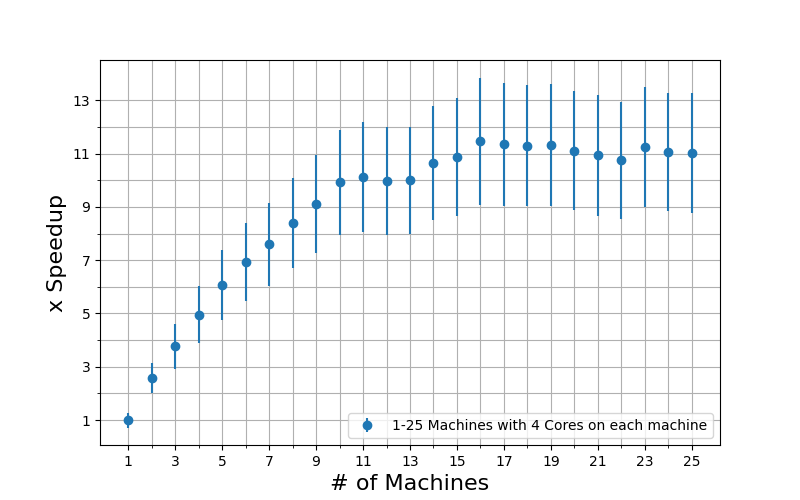
\includegraphics[width=1.0\textwidth, ]{pictures/MachinesXSpeedupWhite.png}
    \caption{The speedup of the Ray implementation with a ninety five percent confidence interval when using one to twenty five machines with \SI{4}{VCPUs/Cores}, relative to using one machine.}
    \label{fig:MachineXSpeedup}
\end{figure}

\cref{fig:MachineXSpeedup} shows the relative speedup of the Ray implementation depending on the number of machines used.
All machines used in the results for \cref{fig:MachineXSpeedup} have 4 VCPUs @ \SI{2.6}{\giga\hertz} and \SI{8}{\giga\byte} memory assigned.
It is odd that between two and nine machine the speedup is larger than the number of machines, for example for five machines the speedup is six times faster.
The speedup is probably larger than the number of machines because of the services Ray run in the background on the cluster.
See \cref{RaySpeedup} for a deeper discussion of \cref{fig:MachineXSpeedup}.

\begin{figure}[H]
    \centering
    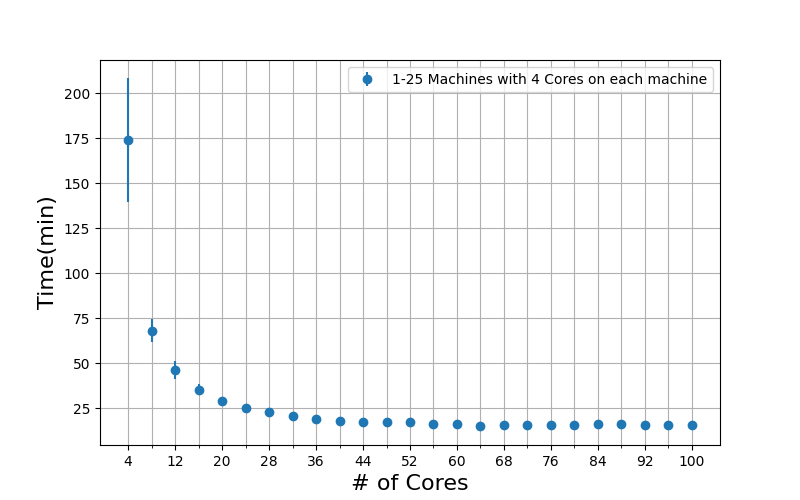
\includegraphics[width=1.0\textwidth, ]{pictures/CoresXTimeMinutesWhite.png}
    \caption{The execution time of the Ray implementation with a ninety five percent confidence interval when using one to twenty five machines with \SI{4}{VCPUs/Cores}.}
    \label{fig:CoresXTime}
\end{figure}

\cref{fig:CoresXTime} shows the total execution time of the Ray implementation depending on the number of cores and indirectly machines.
It is easier to see the diminishing returns for the total execution time each time we add more machines to the problem.


\section{Analysis}

MATLAB is a proprietary interpreted programming language with a heavy focus on matrix operations for use in science, engineering and mathematics.
Python in comparison to MATLAB is an interpreted general purpose language oriented towards the general public.
Python and MATLAB have many things in common but the main difference is the target users, with Python targeting the wider general public and MATLAB targeting scientists and engineers.
Both Python and MATLAB support compilation to speed up code, Python does however have several different implementations of compilers which all focuses on different things.

When it comes to an interpreted language the main issue with speed is that it has to interpret the code at runtime, so it has to read, translate to machine code and execute.
Ignoring the extra overhead from interpreting a program at runtime, compilers also often optimizes things the developer either does not know could be optimized or more often is too lazy to optimize manually.
Compilers can often put the CPU to work in areas of the code where it is idle, it can use caching without explicit use for faster access and performance, reorganize load operations to avoid waiting for the harddrive etc. 
While Python does have many different compilers, the amount of modules in Python are massive and the main problem is that compilers might not support them all.
MATLAB as a proprietary product have an advantage over Python in compiling code as it owns most libraries itself.
It is enormously easier for a development team to maintain and develop a compiler for all libraries in a language if the team develop most libraries itself. 

Even with the many issues in performance with an interpreted language, their scripts tend to be short and the extra execution time is often negligible compared to the extra development time it would take in a lower-level language.
The main advantages with MATLAB is the integrated libraries and the design  which is made specifically for engineers and scientists to reduced development time, according to MATLAB themselves~\cite{WhyMatlab}. 
MATLAB has also shown in multiple other papers to outperform Python in different applications~\cite{EMMatVsPy, ARUOBA2015265}.
Python is however often able to outperform MATLAB when using the right libraries and optimizing the code.
%Refer to own results
Some might argue that the extra development time it would need to optimize the code for some extra speed is why MATLAB is preferable, since all functionality is already integrated.
%To decrease the execution time both MATLAB and Python can use compilers giving about the same execution speeds.
%Above point should have been made in the previous paragraph

Any difference in execution speed is also not the reason why people choose Python or MATLAB, but because of the integrated tools in MATLAB or the flexibility and open-source of Python.
The massive disadvantage of being a propriety product is why more are transitioning to Python.
Open-source means a project such as Python can be developed and criticized by anyone, thus anyone can verify the promises Python makes with their language.
Because MATLAB is proprietary it could be shut down tomorrow, with no more support for it if the company decided so.
Anyone can develop and publish the Python code, while MATLAB is both excluded to those who cannot afford a license and people cannot verify the code of MATLAB, forced to trust the promises of their code.


%(Python and most Python libraries such as NumPy, is open-source which allows anyone to see how it is working under the hood.
%Allowing anyone to see how something is coded means there are more eyes on the code to spot any errors or broken code.
%Python is absolutely free to be distributed and used even commercially.
%Since Python is free it was easier to develop a working product.
%All machine learning algorithms today are almost exclusively written in Python, while not great for the wider market it is something one must account for when using machine learning.
%Python have multiple ways of handling cluster computing which added to the large list of advantages of using Python for this project.)

\section{Conclusion and Discussion}

\subsection{Profiling}

The project has demonstrated the importance of using profiling to find problematic slow running code for improving runtime performance.
After optimization and parallelizing the problem it was possible to decrease the execution time by 200 times using 40 VCPUs. 
The 200 time speedup does not account for the difference in performance for the given hardware, with the results indicating that the VCPUs perform worse individually compared to the test PC.

\subsection{NumPy}

An interesting aspect which was revealed at the end of the project was the fact that a common library such as NumPy was using multiple threads, even in a parallel environment.
The results in this project indicate that the parallelization made in NumPy could be slowing down programs.
Parallel NumPy could maybe be slower due to fighting over resources or communication overhead.
The slower execution time for parallel NumPy could be an array of things and I dare not speculate too much. 
What the slower execution time of parallel NumPy does show is the necessity of profiling and measuring when Python code is meant to be fast.

Python contain so many moving parts, it is impossible to say what implementation will run faster before testing them.
What is usually fastest in Python might be slower due to obscure small things in how they are implemented and used.

\subsection{Python vs. MATLAB}

The project has demonstrated the validity of using Python for science projects and the possibility of translating most MATLAB code to Python.
I do however not recommend translating MATLAB code, I would instead suggest to rewrite the program from scratch with the idea of how it is supposed to work.
The project has highlighted that there are differences even if the vast majority of functions in MATLAB are supported in Python.
Even if most MATLAB functions are supported in Python there are still and will always be libraries with differences, making it almost impossible to achieve identical results.

\subsection{Parallelization}

The project has exposed and showcased the usefulness of utilizing all cores in hardware and the potential speedup of single-thread code.
While not all code exhibit potential parallelism, it can decrease the execution time tremendously when it is possible to parallelize code which exhibits parallelism.

The code could probably see further speedup with a more in-depth analysis of the optimal way to execute it in Ray and by compiling the code.

\subsubsection{Speedup of Ray}\label{RaySpeedup}

The speedup factor in \cref{fig:MachineXSpeedup} is higher than the number of machines for one to ten machines, which is odd.
For example with five machines the speedup factor is around six times faster than using one machine.
The speedup could be larger than the number of machines because of the extra memory added with each node.
More memory means faster access to data, which could speed up computations.
Beside the workload, the master node also hosts the global control store or GCS~\cite{ray:rayCluster,ray:GCS, ray:Architecture}.
The GCS could slow down Ray when using one machine compared to using multiple machines.
There could be a problem with using Ray on only one machine, it is primarily built for a cluster environment and not meant to be used for a single CPU other than for debugging and development.
While the performance gain does decrease with each machine the gain is still quite impressive considering the communication overhead, which can be attributed to the massively parallel problem and almost no serial part in the code.
While Amdahl's law of speedup does not theoretically affect this problem there are issues of the extra overhead with Ray when adding more and more compute nodes, the necessity of keeping everything synchronized and the data transfer of the object store.
The valleys for the speedup factor at around twelve and twenty one machines could be due to the time they were executed, naturally if the scripts are executed during the day the cloud at Ericsson will be at a higher load which could lead to a slowdown.

\subsection{Cloud vs. Local}

The results from \cref{TotTime,Acc:NumPy1Thread} have shown that Cloud solutions might not always be fastest.
However I believe that there are many improvements that can be made in both the Ray and Accelerator implementations to optimize the execution times.
Further work on improving the Ray and Accelerator implementations could perhaps show Ray as being faster.

When the results from both Ray and the Accelerator are on the same order of magnitude it opens the question of what would be optimal for the researchers.
Purchasing a PC with a Xeon or EPYC processor might not be an economically viable option, meaning the renting of a cloud might actually still be preferable.
The Accelerator does have the advantage of maintaining and keeping track of executed code as well as the speedup of skipping already executed code.
It is in the end a discussion the researchers at Lund will have to take themselves.

%Communication overhead? Could be very real since it is probably too divided now
%Unecessary filtration of features with zscore? or faster filtration
%Potential bottleneck in not delaying \texttt{.get} everywhere
%Can it be made faster with more manual spread?
%Bottleneck in permutation, waiting for all to be finished.
%korta ned långa meningar i Matlab koden så den inte hamnar utanför sidan

\section{Outlook}

There are still things which could be improved.
I suspect that at the moment a big reason for the fifteen minute hard limit for the Ray implementation might be due to the high scalability of the current code.
The very smallest parallel code block in the Ray implementation is surprisingly fast to execute.
When the Ray implementation have a growing number of cores and fast small functions, the speed of distributing tasks become increasingly important.
It could be the distribution of small tasks is limiting Ray to utilize the hardware fully.

A suggestion would be to try and divide the code into larger chunks which takes a longer time to execute.
Larger chunks would eliminate some of the communication overhead and Ray would not need to schedule as many tasks.
Too large chunks could however lose too much of the parallelism and bottleneck the code that way instead.
Profiling of the optimal division of chunks would have to be made to see what runs fastest overall, or an in-depth analysis of the optimal number of chunks for the given number of threads.

A problem with the current Ray implementation is the lack of logging and keeping track of what and when something has been executed.
While Ray lack logs the Accelerator lack the scalability of Ray, a future solution could be to have the Accelerator keep track of what and when something has been executed and use Ray to handle the execution.
Some problems would be how to handle setup and remote execution of the code.
The setup of the cluster would probably have to be integrated and executed through the Accelerator.

The advantages are of course the handling of dependencies, possible speedup from skipping unnecessary unchanged parts in the code and the speedup/scalability of Ray.

There is the possibility of developing a custom or another general framework for Ray to track dependencies and accelerating computations.
Because unnecessary features from the Accelerator could be left out from this general framework, it could be faster than integrating Ray and the Accelerator.

The next step in optimizing the MATLAB code would be to integrate the scripts and avoid all unnecessary loading from disk.
It would not change the end result just integrating the scripts more and getting rid of all the intermediate loading of files.
Similiar to the Accelerator an optimization in the MATLAB code could be to create checkpoints which only executes changed code.
The MATLAB code could be tested on octave to integrate it with the Python scripts and run it with Ray for a parallel execution.

\bibliographystyle{vancouver}
\bibliography{reference}

\begin{appendices}

\section{Full Results}

\begin{table}[H]
    \centering
    \begin{tabular}{|l|l|l|}
    \hline
    \#                 & Total (min)        & Speedup AU       \\ \hline
    1 Thread (MAT, PC) & 3426.85$\pm$550.14 & 1.0$\pm$0.23     \\ \hline
    1 Thread (Py, PC)  & 283.63$\pm$1.51    & 12.08$\pm$1.94   \\ \hline
    1 Thread (Py)      & 809.62$\pm$188.22  & 4.23$\pm$1.20    \\ \hline
    true 1 Thread (Py) & 608.48$\pm$42.95   & 5.63$\pm$0.99    \\ \hline
    Ax 4 slices        & 121.77$\pm$13.25   & 28.14$\pm$5.46   \\ \hline
    Ray 1 Nodes        & 174.33$\pm$34.50   & 19.66$\pm$5.01   \\ \hline
    Ray 2 Nodes        & 68.06$\pm$6.55     & 50.35$\pm$9.42   \\ \hline
    Ray 3 Nodes        & 46.29$\pm$5.13     & 74.02$\pm$14.44  \\ \hline
    Ray 4 Nodes        & 35.15$\pm$3.13     & 97.48$\pm$17.89  \\ \hline
    Ray 5 Nodes        & 28.78$\pm$2.46     & 119.09$\pm$21.65 \\ \hline
    Ray 6 Nodes        & 25.10$\pm$1.85     & 136.53$\pm$24.11 \\ \hline
    Ray 7 Nodes        & 22.93$\pm$1.23     & 149.42$\pm$25.28 \\ \hline
    Ray 8 Nodes        & 20.77$\pm$0.64     & 165.02$\pm$26.97 \\ \hline
    Ray 9 Nodes        & 19.12$\pm$0.81     & 179.22$\pm$29.76 \\ \hline
    Ray 10 Nodes       & 17.58$\pm$0.49     & 194.94$\pm$31.76 \\ \hline
    Ray 11 Nodes       & 17.21$\pm$0.75     & 199.09$\pm$33.13 \\ \hline
    Ray 12 Nodes       & 17.49$\pm$0.92     & 195.97$\pm$33.11 \\ \hline
    Ray 13 Nodes       & 17.43$\pm$0.51     & 196.60$\pm$32.09 \\ \hline
    Ray 14 Nodes       & 16.36$\pm$0.60     & 209.52$\pm$34.50 \\ \hline
    Ray 15 Nodes       & 16.05$\pm$0.82     & 213.55$\pm$35.97 \\ \hline
    Ray 16 Nodes       & 15.22$\pm$1.04     & 225.23$\pm$39.28 \\ \hline
    Ray 17 Nodes       & 15.35$\pm$0.73     & 223.20$\pm$37.37 \\ \hline
    Ray 18 Nodes       & 15.43$\pm$0.59     & 222.11$\pm$36.65 \\ \hline
    Ray 19 Nodes       & 15.41$\pm$0.67     & 222.39$\pm$37.00 \\ \hline
    Ray 20 Nodes       & 15.70$\pm$0.61     & 218.29$\pm$36.06 \\ \hline
    Ray 21 Nodes       & 15.94$\pm$1.03     & 214.99$\pm$37.19 \\ \hline
    Ray 22 Nodes       & 16.22$\pm$0.82     & 211.34$\pm$35.59 \\ \hline
    Ray 23 Nodes       & 15.49$\pm$0.41     & 221.24$\pm$36.00 \\ \hline
    Ray 24 Nodes       & 15.77$\pm$0.59     & 217.33$\pm$36.00 \\ \hline
    Ray 25 Nodes       & 15.83$\pm$0.79     & 216.47$\pm$35.84 \\ \hline
    \end{tabular}

    \caption{Table of the total execution times for the all scripts and Ray with 1-25 machines as well as the total comparative speedup factor between the implementations, with 1 Thread (MATLAB) as the default speed.}
    \label{AppendixFullTimeExecSpeedup}
\end{table}


\section{Source Code Repository}

%Replace below FOR GITHUB Link or reference to source code or alternative
\url{https://gitlab.datahub.erdc.ericsson.net/Erickson/masterthesiseeganalysis}

\end{appendices}


\end{document}